% -*- mode: fundamental -*-

% ****************************************************************

\chapter{RISC-V: Drum final topics: traps and interrupts}

\markboth{Ch \arabic{chapter}: Pending (DRAFT)}{\copyrightnotice}

\setcounter{page}{1}
% \renewcommand{\thepage}{\arabic{page}}
\renewcommand{\thepage}{\arabic{chapter}-\arabic{page}}

\label{ch_Drum_Pending}

% ****************************************************************

% ----------------
\vspace{2ex}

\centerline{
\includegraphics[width=1in,angle=0]{Figures/Fig_Under_Construction}}

NOTE:
\fbox{\small
\begin{minipage}{5in}

This chapter is to be written.  The principal topics are:

\begin{tightlist}

  \item Extending RV32I with just enough CSRs and mechanisms to handle traps (for illegal instructions and memory faults)

  \item Extending RV32I to handle timer and external interrupts, so it
  can support an RTOS and perform basic performance measurement.

\end{tightlist}

\end{minipage}}
% ----------------

\begin{figure}[htbp]
  \centerline{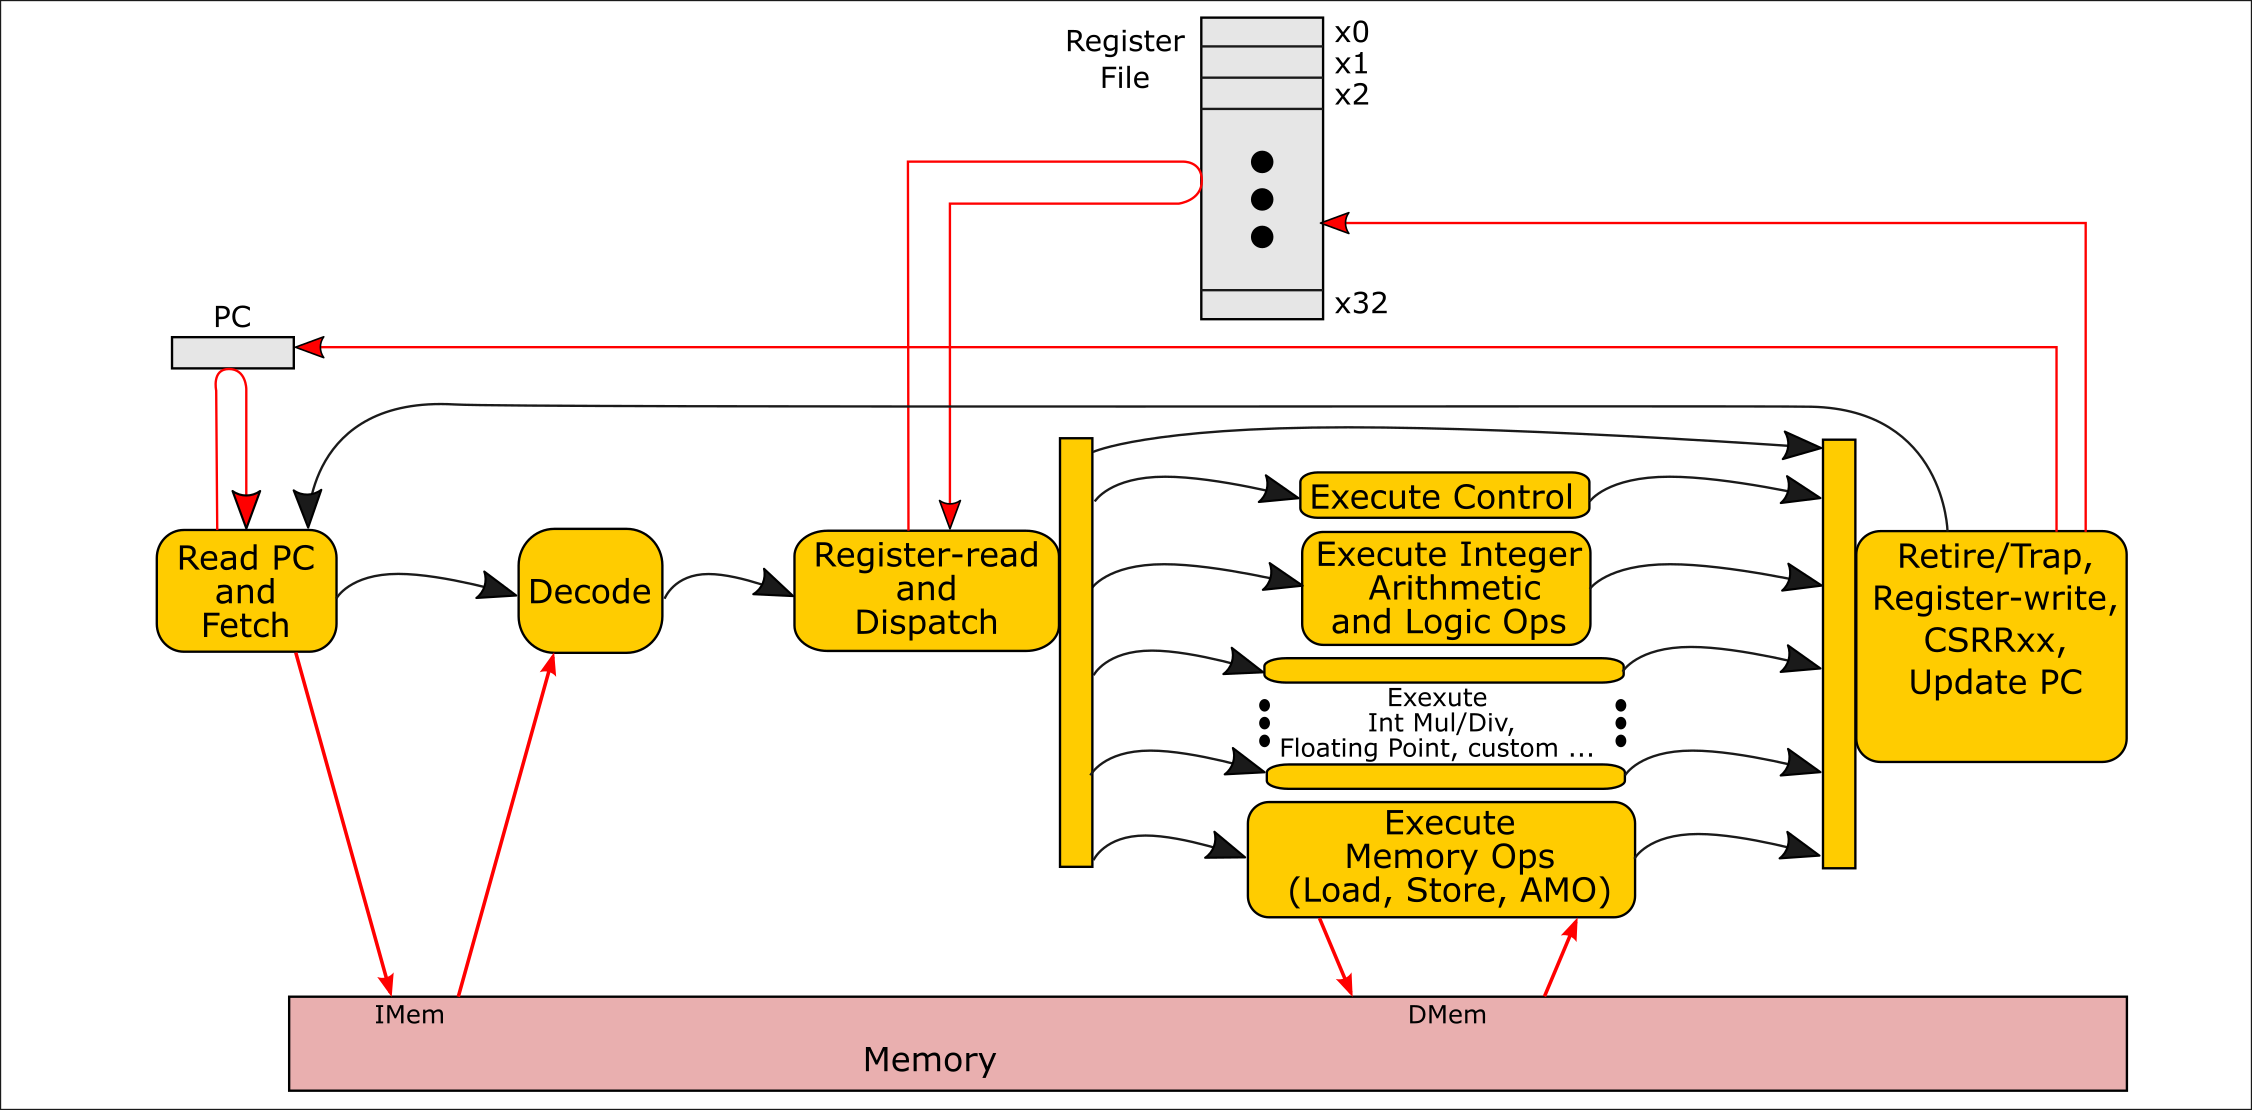
\includegraphics[width=6in,angle=0]{ch030_RISCV_Design_Space/Figures/Fig_Instr_Exec}}
  \caption{\label{Fig_Pending_Simple_Instr_Exec}Simple interpretation of RISC-V instructions (same as Fig.~\ref{Fig_Instr_Exec})}
\end{figure}

\hdivider

% ****************************************************************

\section{Drum: Traps}

Basic overview of how RISC-V does trap-handling is already covered in Chapter~\ref{ch_ISA}.

Here:

\begin{tightlist}

 \item Adding trap-handling CSRs (Control and Status Registers)
     MCAUSE, MTVAL, MEPC, MTVEC, MCAUSE, MRET, minimal MSTATUS.

 \item Adding CSRRxx instructions to access CSRs

 \item Adding trap-handling

\end{tightlist}

% ****************************************************************

\section{Drum: Interrupts}

Interrupts in Drum:
\begin{tightlist}
  \item General concepts: CSRs MIP and MIE; minimal MSTATUS with interrupt-enable bits

  \item Interrupts are initially disabled using the
        MSTATUS.interrupt-enable bit immediately; CSRxx can be used to
        re-enable.

  \item MMIO addresses MTIME, MTIMECMP.  CSRs TIME, MCYCLE

  \item Interrupts are handled just like traps; the only question is:
        when to check for interrupts and respond.

  \item How does MIE bit return to 0?

\end{tightlist}

% ****************************************************************

\section{CSRs for Performance Analysis}

CSRs MTIME, MCYCLE, MINSTRET.

Mention ``hpmcounter'' CSRs for other events.

% ****************************************************************
